\chapter{Results}
%\label{chapter:title}

\section{K-Means}

\subsection{Implementation}
\label{subsection:implementation}

\begin{wrapfigure}[23]{L}{0.4\textwidth}
    \centering
    \resizebox{0.3\textwidth}{!}{
        \begin{tikzpicture}[node distance=2cm]
            \node (in1) [io] {Load points to DPU memory};
            \node (pro1c) [io, below=\vspacing of in1] {Broadcast centroids to all DPUs};
            \node (pro1) [processdpu, below=\vspacing of pro1c] {Initialize cluster sums and cluster counters to 0};
            \node (pro2) [processdpu, below=\vspacing of pro1] {For each point find the nearest centroid};
            \node (pro3) [processdpu, below=\vspacing of pro2] {For each point add features to the appropriate cluster sum and increment the cluster counter};
            \node (pro2c) [processcpu, below=\vspacing of pro3] {Recover and sum the cluster sums and counters from all DPUs};
            \node (pro3c) [processcpu, below=\vspacing of pro2c] {Average the new centroids of clusters};
            \node (dec1) [decision, below=\vspacing of pro3c] {Centroids changed?};
            \node (out1) [stop, below=\vspacing of dec1] {Output centroids};

            \draw [arrow] (in1) -- (pro1c);
            \draw [arrow] (pro1c) -- (pro1);
            \draw [arrow] (pro1) -- (pro2);
            \draw [arrow] (pro2) -- (pro3);
            \draw [arrow] (pro3) -- (pro2c);
            \draw [arrow] (pro2c) -- (pro3c);
            \draw [arrow] (pro3c) -- (dec1);
            \draw [arrow] (dec1) -- node[anchor=east] {no} (out1);
            \draw [arrow] (dec1.east) -- node[anchor=south] {yes} ++(3,0) |- (pro1c.east);

            \background{pro1}{pro1}{pro3}{pro3}{I}{DPU Execution}{yellow!20}
        \end{tikzpicture}
    }
    \caption{\label{fig:KMeansDPU}The K-Means algorithm on DPU}
\end{wrapfigure}

The main workload in K-Means is to measure pairwise distances between each point-centroid pair. Obviously this would be way too slow in floating point arithmetic with DPUs. My approach is instead to do a linear quantization of the data on 15 bits. That is to say the features are mapped linearly to the range [-16385,16384] and encoded as 16-bit integers. The extra bit of leeway is there so that we don't overflow when subtracting features. The entire algorithm is then run in this format, and only at the end the quantized data is converted back to floating point.

This brings two questions. The first one is why choose 16 bits and not 8, since the hardware supports only 8-bit multiplications? Wouldn't that mean that we would end up being 4 times slower than in 8 bits, since performing a 16 bits multiplication with 8 bits hardware needs 4 multiplications? To understand this choice, remember that the DPUs are RISC processors. This means that for each cycle they only execute a very simple instruction. For example, a multiplication needs two load instructions (one for each operand), one multiplication instruction, and one store instruction.

Consider the following simple function to compute the squared euclidean distance between two vectors:
\begin{lstlisting}[language=C]
#include <stdint.h>

int64_t euclid(
    int16_t* a,
    int16_t* b,
    int size
) {
    int64_t accumulate;
    for(int i=0; i<size; i++) {
        volatile int16_t diff = a[i] - b[i];
        accumulate += diff * diff;
    }
    return accumulate;
}    
\end{lstlisting}

Once compiled for DPUs, this function ends up being 26 instructions long. Only 12 instructions are spent on the actual multiplication, and the rest is spent on the subtraction, the loop and the return. If we replace the inputs and the difference with 8-bits integers, the function is now 17 instructions long. All in all, that's only a 60\% performance degradation for more than double the numerical precision, which is quite the trade-off.

The other question is can we trust the algorithm once we've quantized the data? Surely, it is possible to construct a counter-example where the quantization would lead to an incorrect result. However, and allow me to emphasize this, \textbf{floating point K-Means has similar issues, especially in 32 bits}~\cite{jezequel:hal-02486753}. Working in floating point isn't a guarantee against rounding errors, quite the opposite. Working with integers, we can at least be sure that small values don't get rounded to zero when we perform long addition loops.

The important question isn't theoretical, but empirical: does the algorithm generally work on real datasets? We will see that it does.

\bigskip

The implementation is shown in Figure \ref{fig:KMeansDPU}. First, the data on the host is quantized, split (without redundancy) and loaded to the DPUs. Then, the initial random centroids are broadcasted to the DPUs. The DPUs keep a registry of cluster coordinate sums and cluster point count. The DPUs compute the nearest centroid for each point, and adds this point's coordinates to the appropriate cluster sum and increments the cluster point count. Once all the DPUs have returned, the host reads the cluster sums and counts from all DPUs, and aggregates them to compute the new centroid coordinates. The host then compares the new centroid coordinates to the old ones, and if they are different, the centroids are broadcasted and the process is repeated. The process is repeated until the centroid coordinates don't change anymore.

There is one final step omitted for simplicity: the DPUs run one more time to compute the total inertia. This is necessary to select the best clustering when we restart the K-Means algorithm with different initialization.

Do note that, unlike on the CPU implementation, at no point do we keep a list of cluster assignments for the data points, neither in the host nor in the DPUs. The final output is a list of centroids, and not the cluster assignments for the data points. This choice was made because we only set out to study training performances and not inference. By contrast, on the Scikit-learn version, the cluster assignments are returned as well, but that is because the optimized CPU version already needs to compute that list during the training.

\subsection{Results}

\subsubsection{Hardware}

The tests for DPU and CPU are run on a server with an Intel Xeon Silver 4215 processor with 251 GB of RAM. The tests for GPU are run at ETH Zürich on an A100 GPU.

\subsubsection{Datasets}

For benchmarking, we used a mixture of synthetic and real datasets. Synthetic datasets are convenient for scaling up or down the size and dimensionality for benchmarking and profiling purposes. The real dataset offers a guarantee of real-world applicability.

The synthetic datasets are generated using the \verb|make_blobs| function from Scikit-learn. For the weak scaling tests, the datasets have 100,000 samples per DPU, with 16 features grouped into 16 clusters, for a pre-quantization size of 6.4 MB per DPU. For the strong scaling tests, the dataset has 25,600,000 samples total, with 16 features grouped into 16 clusters, for a pre-quantization size of 1.6 GB (halved after 16-bits quantization).

The real dataset is the HIGGS Boson dataset~\cite{baldi2014searching} available at~\cite{Dua:2019}. It has 11 million points, 28 features, and one binary label column that we drop for clustering.

\subsubsection{Weak scaling}

\begin{figure}
    \begin{subfigure}{0.48\linewidth}
        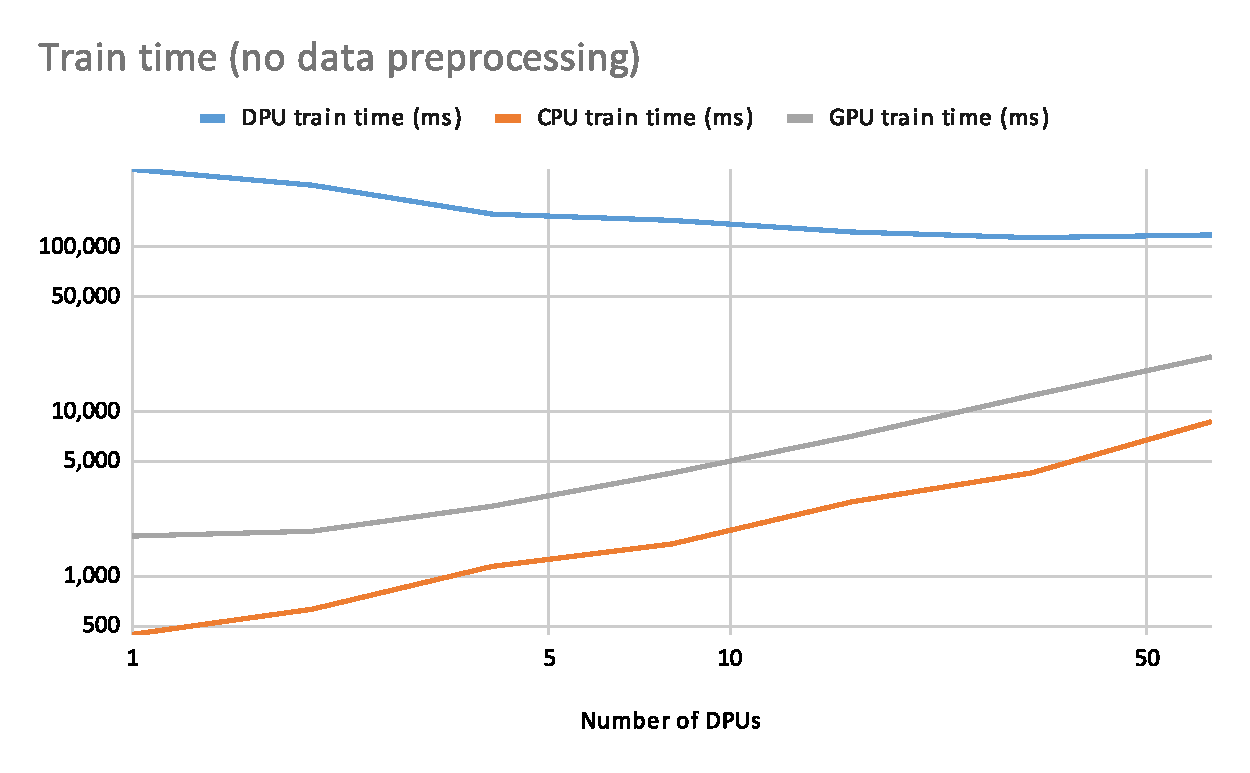
\includegraphics[width=\linewidth]{figures/KMeansweak.pdf}
        \caption{Weak scaling run times for 1 to 64 DPUs}
        \label{fig:KMeansweak}
    \end{subfigure}\hfill
    \begin{subfigure}{0.48\linewidth}
        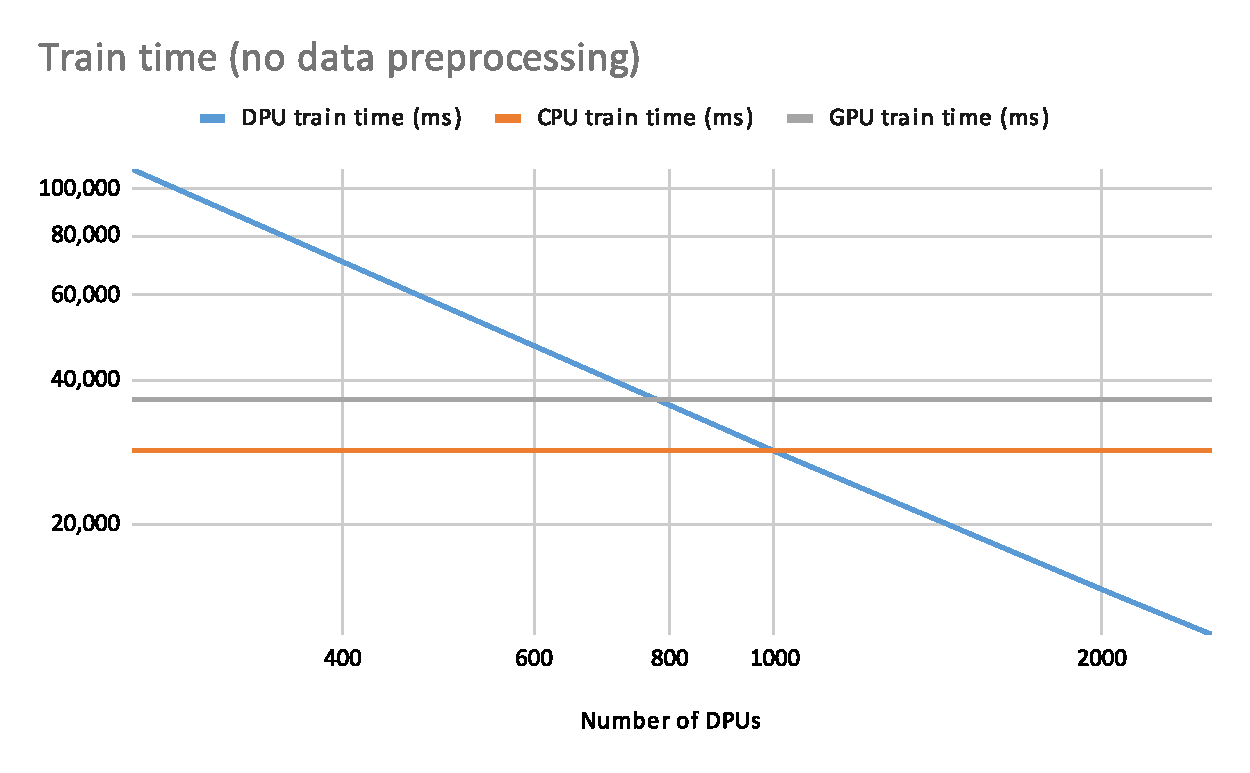
\includegraphics[width=\linewidth]{figures/KMeansstrong.pdf}
        \caption{Strong scaling run times for 256 to 2524 DPUs}
        \label{fig:KMeansstrong}
    \end{subfigure}\par\medskip
    \begin{subfigure}{0.48\linewidth}
        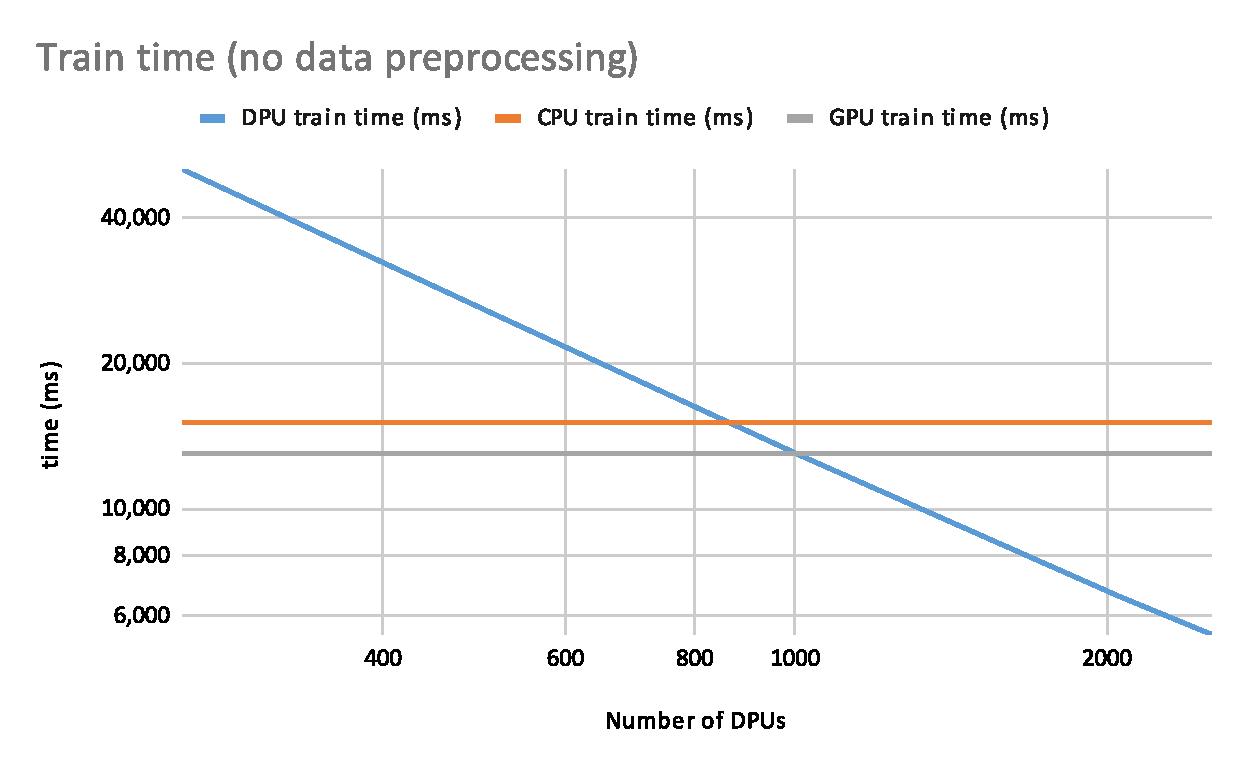
\includegraphics[width=\linewidth]{figures/KMeansHiggs.pdf}
        \caption{Higgs run times for 256 to 2524 DPUs}
        \label{fig:KMeansHiggs}
    \end{subfigure}\hfill
    \begin{subfigure}{0.48\linewidth}
        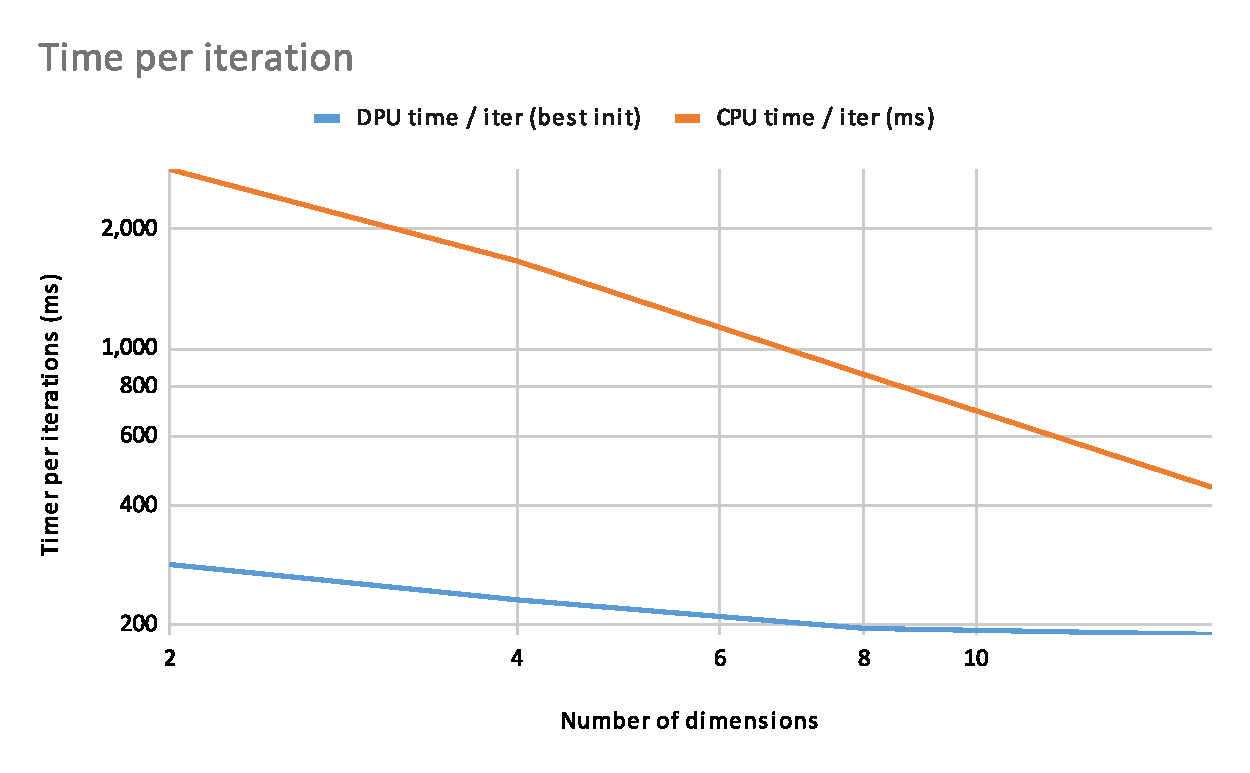
\includegraphics[width=\linewidth]{figures/KMeansdim.pdf}
        \caption{Dimension run times for 2 to 16 dimensions.}
        \label{fig:KMeansdim}
    \end{subfigure}
    \caption{K-Means benchmark results}
\end{figure}

A weak scaling test means that we scale the number of DPUs, and we also scale the dataset size so that the number of points per DPU remains constant.

The results compared to CPU and GPU can be seen on Figure \ref{fig:KMeansweak}. We can see that the processing time remains almost constant with the number of DPUs. It even reduces a little, but that's because K-Means converges in few iterations on smaller datasets. The time per iteration (not shown here) remains perfectly constant.

\subsubsection{Strong scaling}

A strong scaling test means that we scale the number of DPUs, but keep the size of the dataset constant.

The results can be seen on Figure \ref{fig:KMeansstrong}. We can see that we get a perfectly linear scaling of the performance with the number of used DPUs, surpassing the CPU at 1000 DPUs. We can also notice that the GPU is slower than the CPU. It happens on some datasets, depending on their geometry. This is due to the fact that the GPU implementation of K-Means in RAPIDS is batched for internal memory reasons, and thus less numerically stable.

\subsubsection{Higgs}

We run the K-Means algorithm on the Higgs Boson dataset. The performance results can be seen on Figure \ref{fig:KMeansHiggs}. This time the GPU does perform slightly faster than a CPU. UPMEM PIM still outperforms both at 1000 DPUs. The best speedup is achieved at 2524 DPUs with a 2.37x speedup against the GPU.

\subsubsection{Dimensionality}

The dimensionality of the dataset is also a factor in the performance. The results can be seen on Figure \ref{fig:KMeansdim}. We generate datasets of constant size in memory, but with a varying number of features. The best speedup vs CPU is achieved at the lowest dimensionality. We hypothesize that the CPU is more able to take advantage of its vectorization capabilities at higher dimensions, hence the difference. The DPU/CPU performance ratio goes from 10 at 2 dimensions to 1.54 at 16 dimensions.

\subsubsection{Quality}

In section \ref{subsection:implementation}, we discussed the potential precision issues coming from quantization. To assess the quality of the produced results, we used the \verb|Calinski-Harabasz| function from Scikit-learn. The Calinski-Harabasz index~\cite{calinski1974dendrite} is a measure of how well the points are clustered. Unlike the silhouette score, it has a reasonable complexity, so we can use it for large datasets. We also use the adjusted Rand index~\cite{hubert1985comparing} to assess the similarity of the CPU and DPU clusterings.

We find that, for every data set, synthetic and natural, both algorithms always converge to the same minimum. The Calinski-Harabasz are identical within at least 5 significant digits, and the lowest adjusted Rand index in all the tests is 0.99889. This shows that the rounding errors don't cause the DPU implementation to diverge.

\subsubsection{Pipeline occupancy}

We also measured the pipeline occupancy of the DPU kernels. The pipeline occupancy is defined as the number of instructions divided by the number of cycles. It is above 95\%. Along with some profiling on the number of used tasklets, this shows that we are not limited by memory accesses.

\section{Decision Trees}

\subsection{Implementation}
\label{subsection:DTimplementation}

\begin{figure}
    \centering
    \resizebox{0.7\textwidth}{!}{
        \begin{tikzpicture}[node distance=2cm]
            \node (in1) [io] {Load points to DPU memory};
            \node (pro1c) [io, below=\vspacing of in1] {Load an active leaf};
            \node (pro2c) [decision, below=\vspacing of pro1c] {Splits evaluated?};
            \node (pro31c) [processcpu, below left=\vspacing of pro2c] {Add evaluation instruction};
            \node (pro32c) [processcpu, below right=\vspacing of pro2c] {Add commit instruction};
            \node (pro4c) [io, below=2*\vspacing of pro2c] {Transfer instructions to DPUs};
            \node (pro1) [io, below=\vspacing of pro4c] {Load an instruction};
            \node (pro21) [processdpu, below left=\vspacing of pro1] {class count};
            \node (pro22) [processdpu, below right=\vspacing of pro1] {rearrange according to split};
            \node (pro51c) [processcpu, below=\vspacing of pro21] {read results\\evaluate Gini};
            \node (pro52c) [processcpu, below=\vspacing of pro22] {create new leaves};
            \node (pro6c) [decision, below=4*\vspacing of pro1] {Tree finished?};
            \node (out1) [stop, below=\vspacing of pro6c] {Output Tree};

            \draw [arrow] (in1) -- (pro1c);
            \draw [arrow] (pro1c) -- (pro2c);
            \draw [arrow] (pro2c) -- node[anchor=north] {no} ++(-3,0) -| (pro31c);
            \draw [arrow] (pro2c) -- node[anchor=north] {yes} ++(3,0) -| (pro32c);
            \draw [arrow] (pro31c) --  ++(0,-0.75) -| (pro4c);
            \draw [arrow] (pro32c) --  ++(0,-0.75) -| (pro4c);
            \draw [arrow] (pro4c) -- (pro1);
            \draw [arrow] (pro1) -- node[anchor=south east] {evaluate} ++(-3,0) -| (pro21);
            \draw [arrow] (pro1) -- node[anchor=south west] {commit} ++(3,0) -| (pro22);
            \draw [arrow] (pro21) -- (pro51c);
            \draw [arrow] (pro22) -- (pro52c);
            \draw [arrow] (pro51c) --  ++(0,-0.6) -| (pro6c);
            \draw [arrow] (pro52c) --  ++(0,-0.75) -| (pro6c);
            \draw [arrow] (pro6c) -- node[anchor=east] {yes} (out1);
            \draw [arrow] (pro6c.east) -- node[anchor=south] {no} ++(6,0) |- (pro1c.east);

            \background{pro21}{pro1}{pro22}{pro22}{I}{DPU Execution}{yellow!20}
            \background{pro31c}{pro1c}{pro32c}{pro32c}{I}{For all leaves}{orange!20}
            \background{pro51c}{pro51c}{pro52c}{pro51c}{I}{For all leaves}{orange!20}
        \end{tikzpicture}
    }
    \caption{\label{fig:TreesDPU}The Decision Tree algorithm on DPU}
\end{figure}

Unlike in K-Means, we don't need to do any sort of quantization for decision trees. The only operation on features are comparisons, and those can be run very efficiently even on fixed-point hardware (with a pointer trick described in annex \ref{annex:comparison}).

Where we diverge from the Scikit-learn implementation is that sklearn builds decision trees in a depth-first fashion. That is, assuming we do not provide a stopping condition on the total number of leaves in the tree, in which case it switches to a best-first approach. The great thing about this is that if we do not use said condition, there is no interdependency between the leaves. Which means the tree build order does not matter. We can still use stopping criteria like maximum tree depth, minimum number of samples to split, minimum number of samples in a leaf, and minimum impurity decrease.

This allows us to build the tree in a breadth-first fashion. At every iteration, the host looks at every active leaf and decides to do one of three things with it:

\begin{itemize}
    \item Pick a not-yet-evaluated candidate feature for the split, and ask the DPUs ``What are the minimum and maximum values of this feature in this leaf?''
    \item Pick a random threshold between the minimum and maximum, and ask the DPUs ``What are the class counts if we split this leaf with that threshold?''
    \item Decide which split is the most discriminant, add leaves to the current node, and tell the DPUs ``Commit to this split by reorganizing the data belonging to this leaf.''
\end{itemize}

The list of instructions on what to do for each leaf is then sent to the DPUs, which execute them. After they return, the host reads the results and does the appropriate post-processing:

\begin{itemize}
    \item Aggregate the min and max from each DPUs to find the global min and max.
    \item Read the class counts and use it to compute an impurity score.
    \item Decide if the new leaves can be split, or if this branch is finished.
\end{itemize}

This process is illustrated in Figure \ref{fig:TreesDPU}. The algorithm ensures that the data in the DPU memory is always organized according to the tree diagram (i.e. the points belonging to a left node are before the points belong to its sister right node).

The kernel code for the DPUs is quite a bit more complex than in K-Means, and my tutor Julien Legriel wrote the bulk of it when we were pressed for time. It uses streaming memory access to reorganize the data efficiently during a split commit.

\subsection{Results}

\subsubsection{Hardware}

The hardware used for benchmarking is the same as for K-Means.

\subsubsection{Datasets}

As in K-Means, we use both synthetic and real datasets. The synthetic datasets are generated using the \verb|make_classification| function from Scikit-learn. For the weak scaling tests, the datasets have 600,000 samples per DPU, with 16 features in 2 classes, for a size of 38.4 MB per DPU. For the strong scaling tests, the dataset has 153,600,000 samples total, with 16 features in 2 classes, for a size of 9.83 GB.

We also use the Higgs dataset, this time using the target labels for classification, and the last 500,000 samples are reserved for validation.

\subsubsection{Weak scaling}

\begin{figure}
    \begin{subfigure}{0.48\linewidth}
        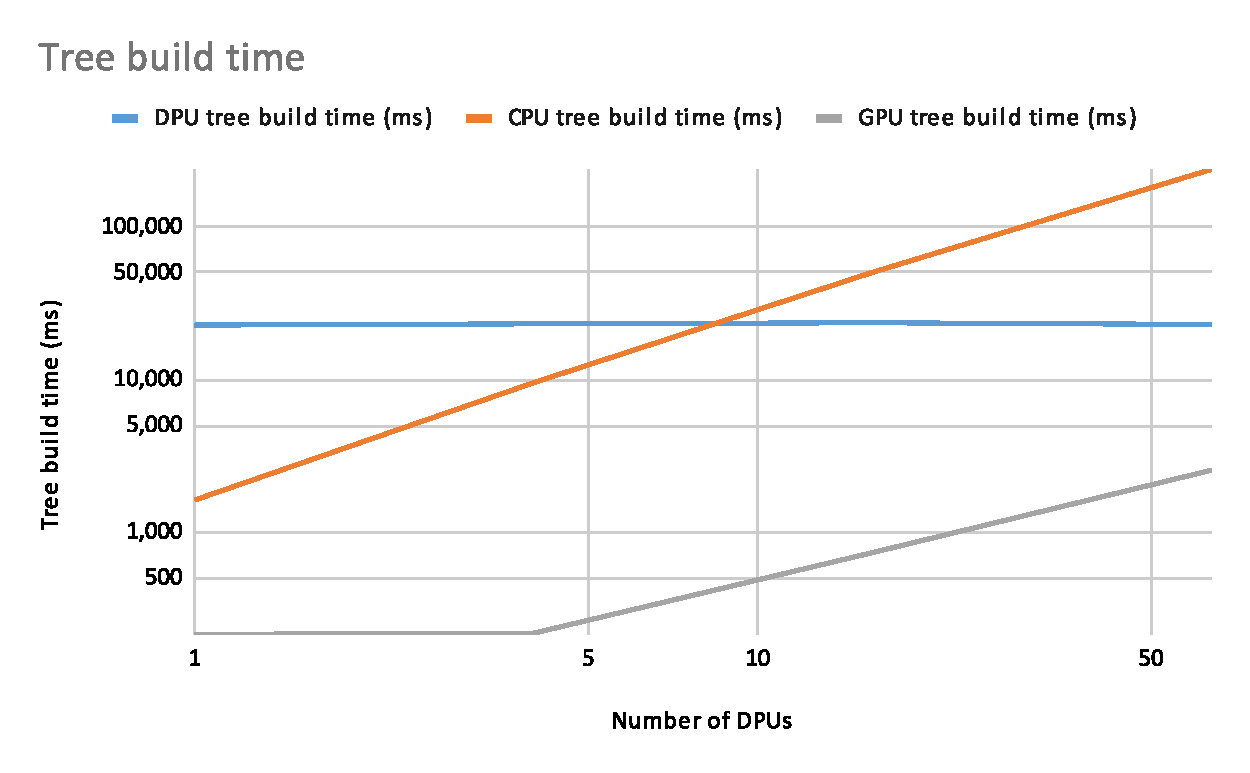
\includegraphics[width=\linewidth]{figures/Treesweak.pdf}
        \caption{Weak scaling run times for 1 to 64 DPUs}
        \label{fig:Treessweak}
    \end{subfigure}\hfill
    \begin{subfigure}{0.48\linewidth}
        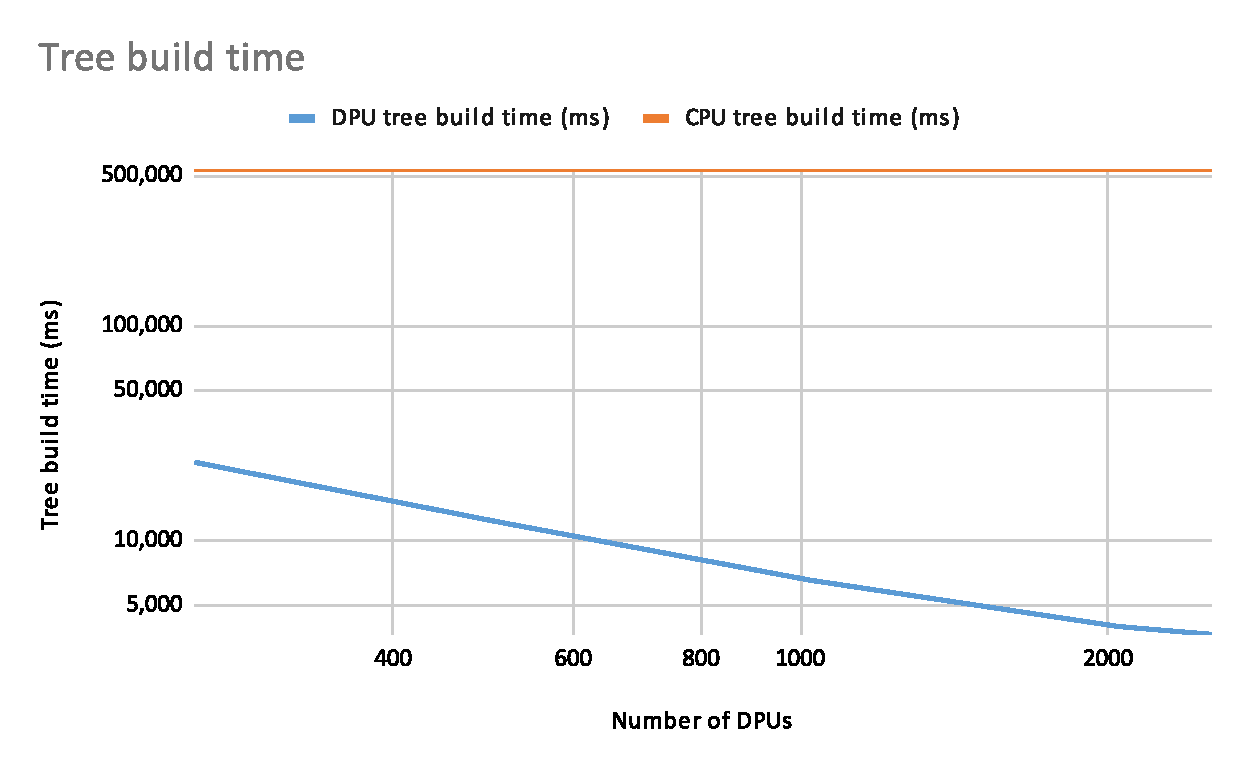
\includegraphics[width=\linewidth]{figures/Treesstrong.pdf}
        \caption{Strong scaling run times for 256 to 2524 DPUs}
        \label{fig:Treesstrong}
    \end{subfigure}\par\medskip
    \begin{subfigure}{0.48\linewidth}
        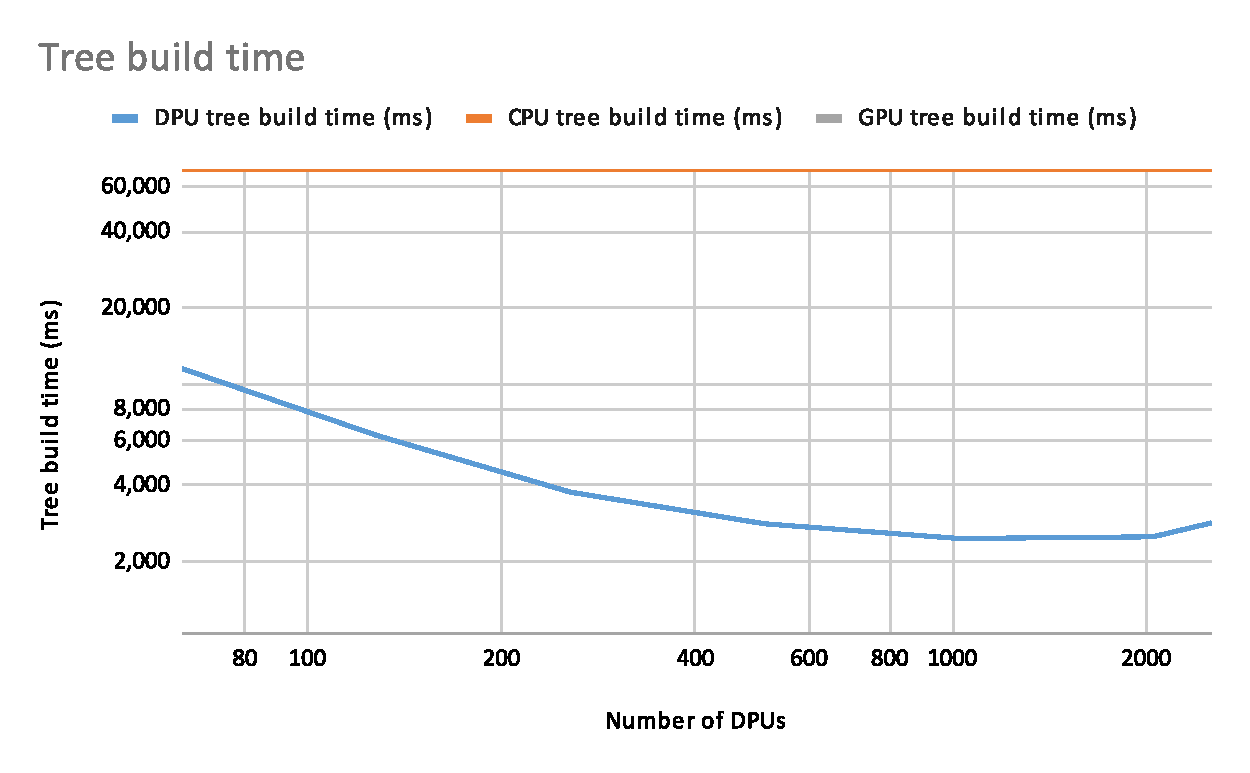
\includegraphics[width=\linewidth]{figures/TreesHiggs.pdf}
        \caption{Higgs run times for 256 to 2524 DPUs}
        \label{fig:TreesHiggs}
    \end{subfigure}\hfill
    \begin{subfigure}{0.48\linewidth}
        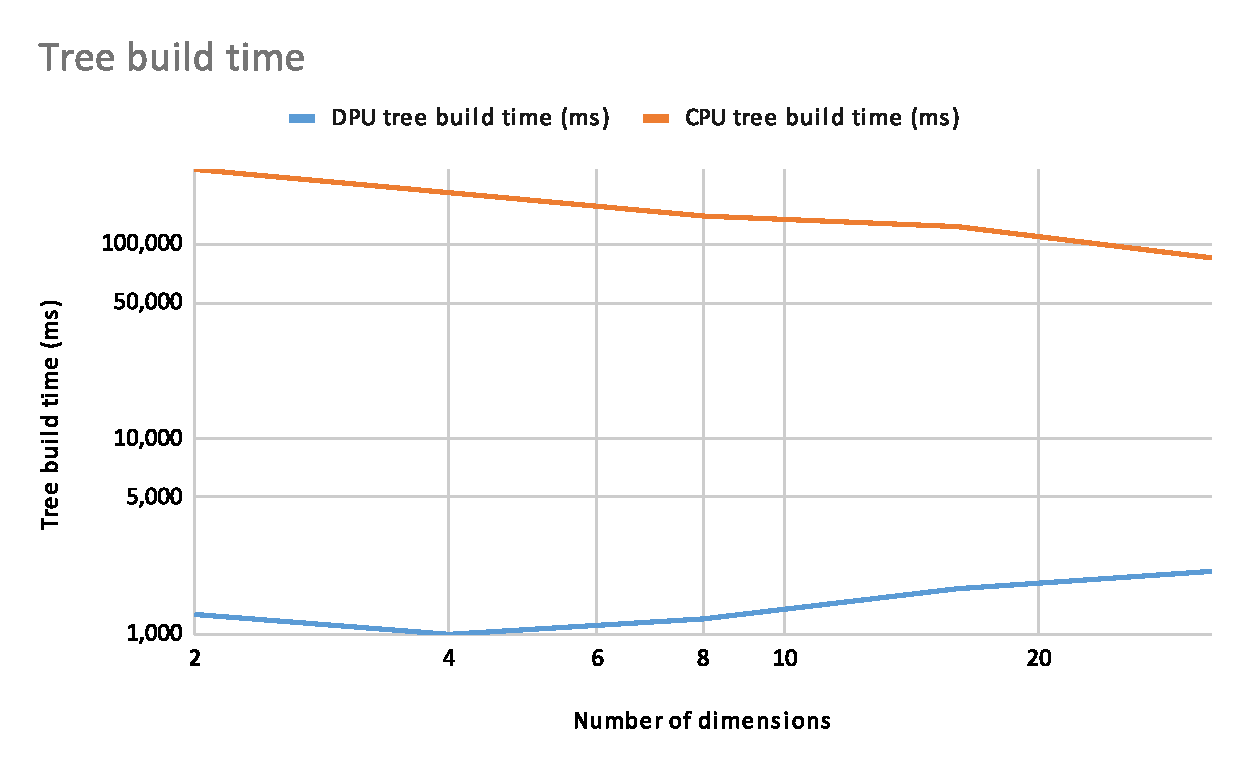
\includegraphics[width=\linewidth]{figures/Treesdim.pdf}
        \caption{Dimension run times for 2 to 24 dimensions.}
        \label{fig:Treesdim}
    \end{subfigure}
    \caption{Decision Trees benchmark results}
\end{figure}


We can see in Figure \ref{fig:Treessweak} that the DPU execution time is perfectly constant.

\subsubsection{Strong scaling}

We can see in Figure \ref{fig:Treesstrong} that the performance gain with the number of CPUs is roughly linear. It does start to saturate after 1024 DPUs. Do note that there is no GPU comparison for this benchmark. The GPU can load the dataset in memory, but doesn't have enough space left to perform the computation.

\subsubsection{Higgs}

Unfortunately, we see in Figure \ref{fig:TreesHiggs} that our DPU system reaches saturation before outperforming the GPU. The Higgs dataset is just too small for us to take advantage of the architecture. Nevertheless, we won't go cherry-picking\footnote{The practice of pointing only to data that seems to confirm a particular hypothesis.} here just to find a dataset that shows the results we want. 

\subsubsection{Dimensionality}

Figure \ref{fig:Treesdim} shows that there is also a dimensionality effect at play here. We go from a 191 speedup factor in dimension 2 to 40 in dimension 32. This is harder to explain, we hypothesize that it is due to the fact that a higher dimension means we have to make more, shorter, back-and-forth iterations between the host and DPUs.

\subsubsection{Quality}

Although our implementation is functionally identical with the Scikit-learn version, there is one difference coming from the fact that we don't build tree leaves in the same order. Because this is a probabilistic algorithm, the random number generation ends up being different. So to compare the two, we run the algorithms several times with different seeds and compare the accuracies. This time, this is simply a sanity check on our implementation.

On ten runs on one DPU with 600,000 samples, the mean accuracies for DPU and GPU are 0.90008 and 0.90175 respectively, and the covariance between the two series is 1.39E-4. This confirms our implementation is correct outside of extreme edge cases.

\subsubsection{Pipeline occupancy}

Perhaps more surprisingly this time, pipeline occupancy and tasklets profiling reveals that we are still not memory-bound, despite this algorithm being much less computationally intensive than K-Means. This is good news for the scalability of the algorithm.